\subsection{Subpaso 2-A: Ingresar sanción para el solicitante}	
	Para la sanción del solicitante se mostrará la interfaz 
	
	\begin{figure}[hbtp]

	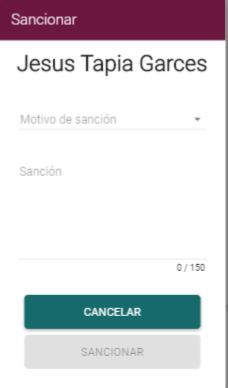
\includegraphics[scale=0.3]{images/InterfazMovil/IUGS07_sancionarSolicitante.PNG}
	\caption{Sancionar Solicitante}
	\end{figure}
	
	 Se	deberá seleccionar una de las opciones por la cual 
	ha sido el solicitante sancionado y la descripción 
	de la misma.	
	\begin{enumerate}
		\item seleccione motivo de la sanción.
		\item Ingrese la descripción de la sanción. \textbf{(Veáse error ER01)}
		\item presiona el botón \textbf{Sancionar}. 
	\end{enumerate}
		\begin{figure}[hbtp]

	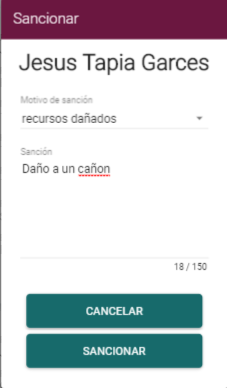
\includegraphics[scale=0.3]{images/InterfazMovil/IUGS07_sancionarSolicitanteBoton.PNG}
	\caption{Sancionar Solicitante}
	\end{figure}
		
	Cuando al sanción se haya registrado se mostrará el siguiente mensaje:
	\textit{Usted se encuentra sancionado por [motivo] y debe cumplir con 
	[penalización]. [Si existe, mostrar duración de la sanción]. Diríjase al DAT 
	para mayor información. }
	
	\textbf{Observación 1.} El solicitante no debe tener 
		una reservación hecha previamente, en caso contrario, 
		esta se cancelará.
	
\subsection{Subpaso 2-B: ER01. Los datos no han sido llenados correctamente}
	Se mostrará el siguiente mensaje cuando todos los campos no hayan
	llenados. \par	
	\textit{No se han llenado todos los campos del formulario}\par
	Se deberán ingresar todos los campos para continuar con la sanción.
	
	
	